% $Header: /cvsroot/latex-beamer/latex-beamer/solutions/conference-talks/conference-ornate-20min.en.tex,v 1.6 2004/10/07 20:53:08 tantau Exp $

\documentclass[aspectratio=169,9pt,mathserif]{beamer}

\graphicspath{{../}}
%\mode<presentation>
%{
% 
%\usetheme{Montpellier}
  \usetheme[compress,mathserif]{Hannover}%Dresden}%
  % or ...
\usefonttheme{structurebold} 

\setbeamertemplate{Hannover}{sidebar your definition}

  \setbeamercovered{transparent}
  % or whatever (possibly just delete it)
    \definecolor{mblue1}{rgb}{0., 0.1, 0.95}
%        \definecolor{mblue1}{rgb}{0.5, 0.5, 0.7}
    \definecolor{mblue}{rgb}{0.35, 0.7, 0.7}%        \definecolor{mblue}{rgb}{0.55, 0.85, 0.85}
%                \definecolor{mblue}{rgb}{0.4, 0.55, 0.9}
    \definecolor{mgrey}{rgb}{0.7421875,0.7421875,0.7421875} 

  \usecolortheme{dove}

  \usenavigationsymbolstemplate{}
 % \logo{\includegraphics[width=.2\textwidth]{logo-inria-bordeaux.eps}}
 \setbeamercolor*{title}{fg=mblue1, bg=white} 
  \setbeamercolor*{frametitle}{fg=mblue1, bg=white} 
%   \setbeamercolor{normal text}{fg=mblue} 
     \setbeamercolor{structure}{fg=mblue1} 
     \setbeamercolor{block}{fg=mblue1}
\setbeamercolor{block title alerted}{fg=mblue1}

\usepackage[subdued]{mathastext}
\MTfamily{augie}
\Mathastext[augie]

\setbeamerfont{author}{size=\fontsize{10pt}{12pt}}

\setbeamerfont{institute}{size=\fontsize{8pt}{10pt}}
%   \setbeamercolor{navigation symbols}{fg=mblue} 
%   \setbeamercolor{section in sidebar shaded}{fg=mblue}
%   \setbeamercolor{palette sidebar secondary}{fg=mblue}   
\makeatletter
   \setbeamertemplate{sidebar canvas \beamer@sidebarside}%
                  [vertical shading][top=mblue1,bottom=mblue1]
\makeatother
%}

\usepackage[absolute,overlay]{textpos}	
\setlength{\TPHorizModule}{1mm}
\setlength{\TPVertModule}{1mm}
\newcommand{\MyLogo}{%
%\begin{textblock}{14}(66,60)%(113.4,0.7)
%  \includegraphics[width=3.cm,angle=-90]{../honom-logo}
% \end{textblock}
% \begin{textblock}{14}(89,39.7)%(113.4,0.7)
%  
\includegraphics[width=1.7cm,angle=00]{./LOGOS_pack_bureautique/png/inr_logo_noir}
% \end{textblock}

}

\newcommand{\hh}{\mathrm{h}}

\newcommand{\MyLogoa}{%
 \begin{textblock}{14}(0.65,83.)%(113.4,0.7)
  
\includegraphics[width=1cm,angle=00]{logos-Inria-UMA} 
 \end{textblock}

}



\usepackage{graphicx,epsfig,media9,animate}
\usepackage[normalem]{ulem}                             % testo barrato
\newcommand{\stkout}[1]{\ifmmode\text{\sout{\ensuremath{#1}}}\else\sout{#1}\fi}
\usepackage{amsmath,amsfonts,psfrag,amsthm,pstcol,soul,cancel,movie15}
\usepackage{pgf}
\usepackage{xcolor}
\usepackage{wasysym,pifont}
\definecolor{DarkGreen}{rgb}{0.,0.5,0.}

\usepackage[english]{babel}

\usepackage{amsmath,amsfonts}

\newcommand{\F}{\boldsymbol{\mathcal{F}}}
\newcommand{\HH}{\mathcal{H}}
\newcommand{\G}{\mathcal{G}}
\newcommand{\VV}{{\bf V}}
\newcommand{\CN}{\mathcal{CN}}
\newcommand{\Dj}{\mathcal{D}_j}
\newcommand{\Dk}{\mathcal{D}_k}
\newcommand{\Tau}{\mathcal{T}}
\newcommand{\U}{{\bf u}}
\newcommand{\PRi}{{\bf p}}
\newcommand{\W}{{\bf w}}
\newcommand{\ST}{\boldsymbol{\mathcal{S}}}
\newcommand{\PP}{\boldsymbol{\Phi}}
\newcommand{\BB}{\boldsymbol{\beta}}
\newcommand{\V}{{\bf v}}
\newcommand{\RD}{\mathcal{RD}}
\newcommand{\CRD}{\mathcal{CRD}}
\newcommand{\QRD}{\mathcal{QRD}}
\newcommand{\LP}{\mathcal{LP}}
\newcommand{\Di}{\mathcal{D}_i}
\newcommand{\PG}{\mathcal{PG}}

\newcommand{\Remi}{{\Large \bf Modif by Remi}}
\newcommand{\Eremi}{{\Large \bf end of modifs}}
\newcommand{\remi}[1]{\emph{#1}}
\newcommand{\dpar}[2]{\dfrac{\partial #1}{\partial #2}}
\newcommand{\modif}[1]{\textcolor{red}{#1}}
\newcommand{\Int}{\displaystyle \int}
\newcommand{\Sum}{\displaystyle \sum}
%
% new commands
%
\newcommand{\Fsc}{\mathcal{F}}
\newcommand{\PR}{{\bf p}}
\newcommand{\Cj}{\mathcal{C}_j}
\newcommand{\Ck}{\mathcal{C}_k}
\newcommand{\Z}{{\bf z}}
\newcommand{\STsc}{{\mathcal{S}}}
\newcommand{\sysPP}{{\pmb \phi}}
\newcommand{\sysbeta}{{\pmb \beta}}
\newcommand{\vki}{von Karman Institute for Fluid Dynamics}
\newcommand{\DG}{\mathcal{DG}}
\newcommand{\FV}{\mathcal{FV}}
\newcommand{\FE}{\mathcal{FE}}
\newcommand{\FS}{\mathcal{FS}}
\newcommand{\Mo}{\mathcal{M}}
\newcommand{\MU}{\mathcal{MU}}
\newcommand{\Ci}{\mathcal{C}_i}
\newcommand{\CL}{\mathcal{CL}}




\title[WENO-FD-GFq] % (optional, use only with long paper titles)
{\textcolor{white}{mm}\\[-0.25cm] Discrete well-balanced WENO finite difference schemes: \\ global-flux quadrature method with multi-step ODE integrator weights} 



\author[Kazolea, Par\'es, Ricchiuto]{Maria Kazolea$^*$, Carlos Par\'es$^+$, Mario Ricchiuto$^*$\vspace{0.1cm} }
\institute[INRIA] % (optional, but mostly needed)
{$^*$Team CARDAMOM,  Inria research center at University of Bordeaux (France)\\[5pt]
$^+$ EDANYA Group, Universidad de M\'alaga (Spain)\\[100pt]
\textcolor{white}{mm}} 


\date{}
 

%
%\date[HONOM 2022] % (optional, should be abbreviation of conference name)
%{HONOM22 \\   April  4th - 8th, 2022 Braga (Portugal)}


	
\subject{Applied Math}

\newcommand\Figref[1]{figure~\ref{#1}} 
\newcommand\secref[1]{\S\ref{#1}}
\newcommand\Ltwo[1]{\| #1 \|_{L^{2}(\Omega)}}
\newcommand{\R}{\mathbb{R}}
\DeclareMathOperator{\dist}{dist}
\DeclareMathOperator{\diver}{div}
\DeclareMathOperator{\diag}{diag}
\newcommand{\id}{\mathrm{Id}}
\DeclareMathOperator{\sign}{sign}
\newcommand{\flux}{\boldsymbol{\mathcal{F}}}
\newcommand{\source}{\boldsymbol{\mathcal{S}}}
\newcommand{\vu}{\mathbf{u}}
\newcommand{\vw}{\mathbf{w}}
\newcommand{\vv}{\mathbf{v}}
\newcommand{\vl}{\mathbf{l}}
\newcommand{\vr}{\mathbf{r}}
\newcommand{\vphi}{\boldsymbol{\phi}}
\newcommand{\vbeta}{\boldsymbol{\beta}}
\newcommand{\vPhi}{\boldsymbol{\Phi}}
\newcommand{\vvarphi}{\boldsymbol{\varphi}}
\newcommand{\eG}{\mathcal{G}}
\newcommand{\eH}{\mathcal{H}}

\newcommand{\speed}{\vec u}
%
%
%
\newtheorem{proposition}{Proposition}[section]
\newtheorem{remark}[proposition]{Remark}


\begin{document}

%Well balanced DG-SEM for systems of balance laws via global fluxes
%
%
%We investigate the construction of well balanced methods based on the notion of a global flux.
%This notion arises naturally in some discretization approaches as e.g. residual distribution,
%and is inherent to some well balanced schemes based on  formulations including augmented
%set of variables including external data (bathymetry for the shallow water equations,
%gravitational potential for the Euler  equations, etc.). Explicit approximations of a global flux via
%quadrature of the source term  have been recently proposed to enhance the well balanced character of
%finite volume methods.   We review briefly this method and we propose a different formulation in the context of notal  DG-SEM methods.
%The collocated nature of the method allows to simplify somewhat  the global flux formulation, while
%still providing a considerable enhancement of the well balanced character of the method for non-trivial equilibria.
%In the talk we discuss the basic formulation,  and provide  some ideas for enhancements including the exact preservation of some
%steady states, and the preservation of and energy/entropy equality.
%Examples for shallow water floes, and  Euler equations with gravitational potential are provided.


%
%
% TITLE SLIDE........
%
%
 
\begin{frame} 

  \titlepage
  
  \vspace{-2cm}
  \MyLogo
    \MyLogoa
  
  \vspace{-1.5cm}
    
    \begin{flushright}
  \textrm{ Converence name\\
Conference adress\\
Conference date}
  \end{flushright}
  
\end{frame}

 
\section[Intro]{Objectives of this work}



\begin{frame}[t]{Setting: balance laws}
\MyLogoa

\vspace{0.5cm}

We want to solve numerically  hyperbolic systems of balance laws

\begin{equation}
	\partial_tU+ \partial_x F(U)=  S(U)\partial_xH \nonumber
\end{equation}
 
\vspace{1.cm}

Typical examples  that we will use here


\begin{itemize}
\item Burger's equations 
\vspace{0.2cm}
\item Shallow water equations with topography
%\only<2->{\item{\bf Shallow water equations with topography/friction/Coriolis/etc}}
\end{itemize}

%\vspace{0.5cm}

% \flushright{\underline{We  consider both 1D and Multi-D problems}}
%\only<1>{\color{white}{\\[5pt] But for simplicity the discussion is done for the 1D case}}
%\only<3>{\\[5pt]But for simplicity the discussion is done for the 1D case}
\end{frame}
 

\begin{frame}[t]{Setting: balance laws}
\MyLogoa

\vspace{0.5cm}

We want to solve numerically  hyperbolic systems of balance laws

\begin{equation}
	\partial_tU+ \partial_x F(U)=  S(U)\partial_xH \nonumber
\end{equation}
 
 
 \vspace{0.5cm}

Shopping list


\begin{itemize}
\item Arbitrary high order
%\only<2->{\item{\bf Shallow water equations with topography/friction/Coriolis/etc}}
\item  Possibly monotonicity/positivity preserving  
%\only<2->{\item  Euler equations with gravity  $\leftarrow$ {\it and  some preliminary results here}  }
\item Steady state preserving 

\end{itemize}

\vspace{0.2cm}

  
 \end{frame}



\begin{frame}[t]{Objective}
\MyLogoa

\vspace{0.5cm}

We want to solve numerically  hyperbolic systems of balance laws

\begin{equation}
	\partial_tU+ \partial_x F(U)=  S(U)\partial_xH \nonumber
\end{equation}
 
 
 \vspace{0.5cm}
\begin{description}
	\item[The objective]  of well balanced schemes is to preserve exactly or with enhanced accuracy some of the steady state
	solutions.
	\vspace{0.1cm}
	\item[We focus] here on the development of well-balanced high order FD methods for general systems of balance laws that preserve all the stationary solutions.  
\end{description}


%Steady state preserving: on a given mesh we want to the scheme embed in the discretization a
%
%\begin{description} 
%
%\vspace{0.2cm}
%
%\item[{\it Definition}] of    $\partial_x F_{\textrm{h}} = S_{\textrm{h}}$ such that data  verifying it is exactly preserved
%
%\vspace{0.2cm}
%
%\item[{\it Projection}]    operator 
%providing such data, possibly different from the scheme
%
%\vspace{0.2cm}
%
%\item [{\it Characterization}]  of the above projection: e.g  enhanced consistency, well posedness 
%\end{description}
 
\end{frame}




\begin{frame}{Some approaches in the Bibliography  for 1D}
\MyLogoa

There are numberless approaches, and vast literature.
Related work:

\begin{enumerate}

\vspace{0.5cm}

\item Reconstruction/evolution of fluctuations wrt  discrete equilibria ({\bf approximate  full well balanced}):

\begin{itemize}
\item {\scriptsize    Castro \& Par\'es J.Sci.Comp. 2020,   G\'omez-Bueno et al, Appl.Math.Comp. 2021,   G\'omez-Bueno et al  athematics 2021,
Guerrero Fern\'andez et al  Mathematics 2021,   G\'omez-Bueno et al, Appl.Num.Math.  2023, etc. etc.}
\end{itemize}

\vspace{0.5cm}


\item Well balanced via integration of the source term and  global fluxes 

\begin{itemize}
\item {\scriptsize   Gasc\'on  \& Corber\'an  JCP 2001,  Donat \& Martinez-Gavara   J.Sci.Comp. 2011, 
Chertock et al JCP 2018, Cheng et al J.Sci.Comp. 2019, Mantri\&Noelle   JCP  2021,  
Ciallella et al.   J.Sci.Comp. 2023,   Xu and Shu J.Sci.Comp. to appear, etc. etc.} 
\end{itemize}

\vspace{0.5cm}


\item  Other approaches 

\begin{itemize}
\item Well balanced via reconstruction/evolution of fluctuations wrt to a given equilibrium
\item Preserving $V(u,\phi(x))=V_0$ via WB differencing or generalized polynomial approximations
\item Fully well balanced Riemann solver with 0-wave to enforce integral steady balance. 
\end{itemize}


\end{enumerate}


\end{frame}
 
 






\section[WENO GFq]{Global flux quadrature for WENO finite difference}


\begin{frame}[t]{
\includegraphics[width=0.3cm]{circle1} Global Flux Quadrature  with WENO approximation} 
\MyLogoa

 We seek solutions of the hyperbolic system of balance laws

\begin{equation}
	\partial_tU+\partial_x F(U)=  S(U)\partial_xH   \nonumber
	\vspace{0.25cm}
\end{equation}


{\bf \textsf{Approach 1.}\footnote{M. Ciallella, D. Torlo, MR, Arbitrary High Order WENO Finite Volume Scheme with Flux Globalization for Moving Equilibria Preservation,  {\it J.Sci.Comp.} 96, 2023 }} 

\only<1-2>{ \begin{equation*} 
 \dfrac{d\overline{U}_i}{dt} + \dfrac{1}{\Delta x} \left( \widehat{G}_{i+1/2} - \widehat{G}_{i-1/2}   \right)   = 0  \nonumber
 \vspace{0.35cm}
\end{equation*}}
 
 \only<2>{
 
 \begin{enumerate}
 \item  Reconstruct  WENO polynomials  ${\color{red}U_i(x)}$
 
 \vspace{0.175cm}
 
 \item  Compute  cell averaged source primitive $ \overline{R}_i =R_{i-1/2}^+ - \sum_q \omega_q  \int_{x_{i-1/2}}^{x_q} S({\color{red}U_i(x)},\varphi(x)) dx$
 
  \vspace{0.1cm}
  
   \item  Compute  cell averaged fluxes  $ \overline{F}_i =  \sum_q \omega_q F({\color{red}U_i(x_q)},\varphi(x_q)) dx$
 
  \vspace{0.175cm}
  
 \item  Reconstruct  WENO polynomials  $G_i(x)= (F+R)_i(x)$ 
 
  \vspace{0.175cm}
  
 \item  Compute upwind fluxes $\widehat{G}_{i+1/2} = (A^+A^{-1})_{i+1/2} G_{i}(x_{i+1/2}) + (A^-A^{-1})_{i+1/2} G_{i+1}(x_{i+1/2})$
 \end{enumerate}
 }

\only<3>{
\vspace{-0.5cm}
\begin{center}
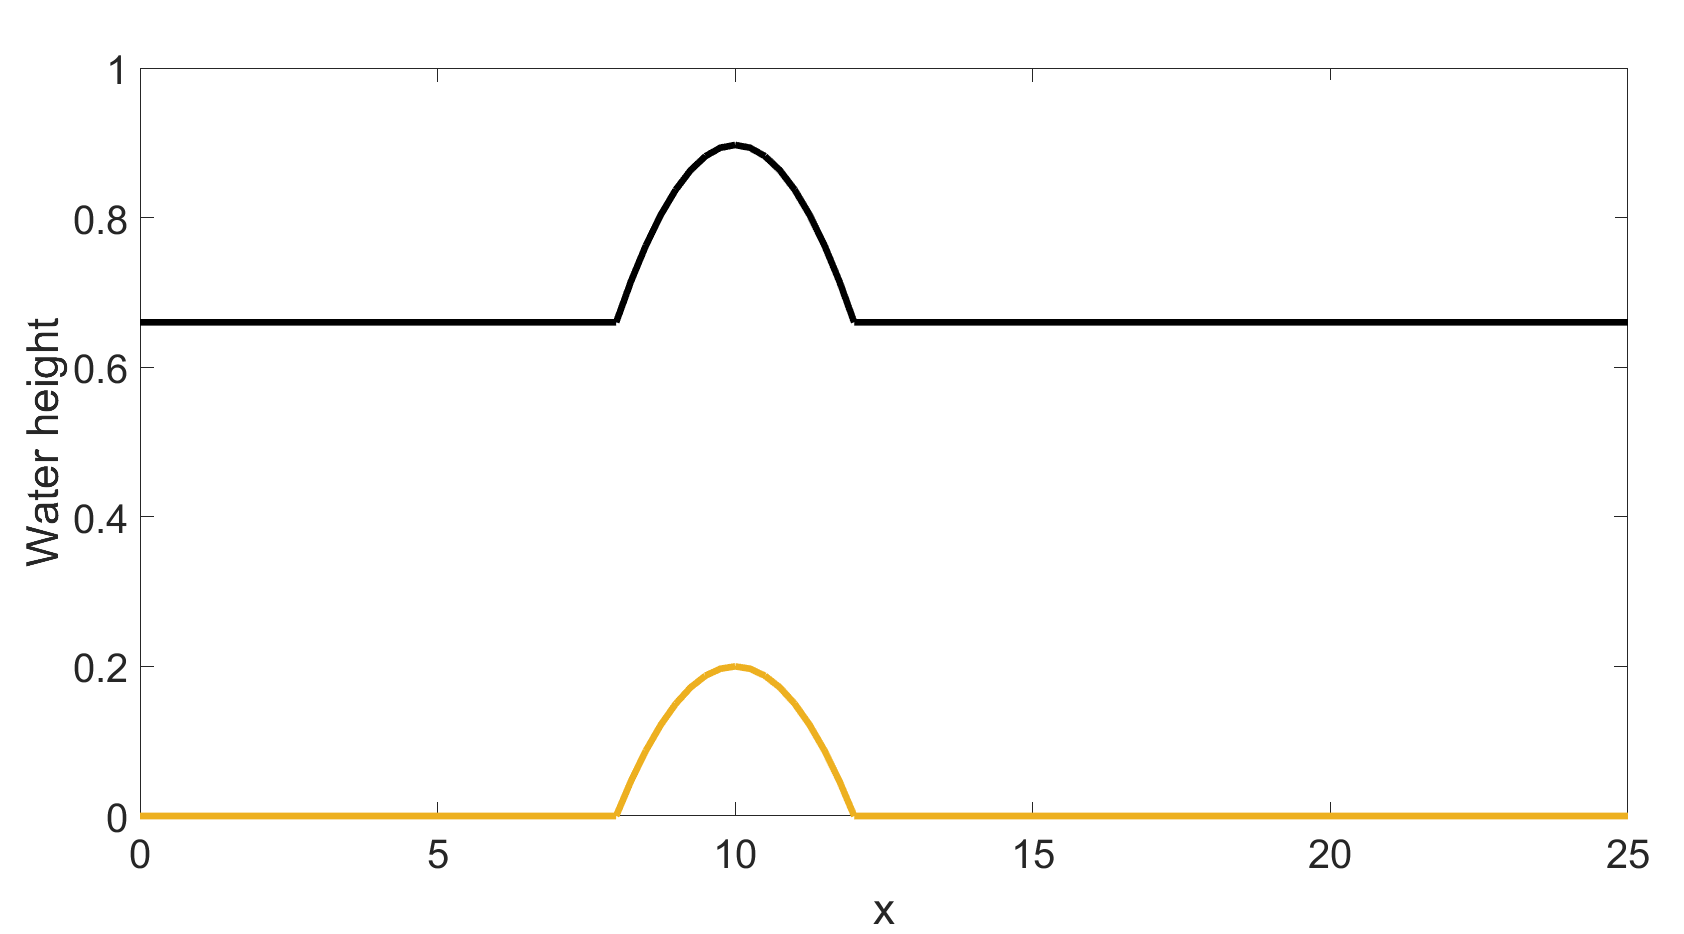
\includegraphics[width=3.5cm,height=1.25cm]{./height_supercrit}\\
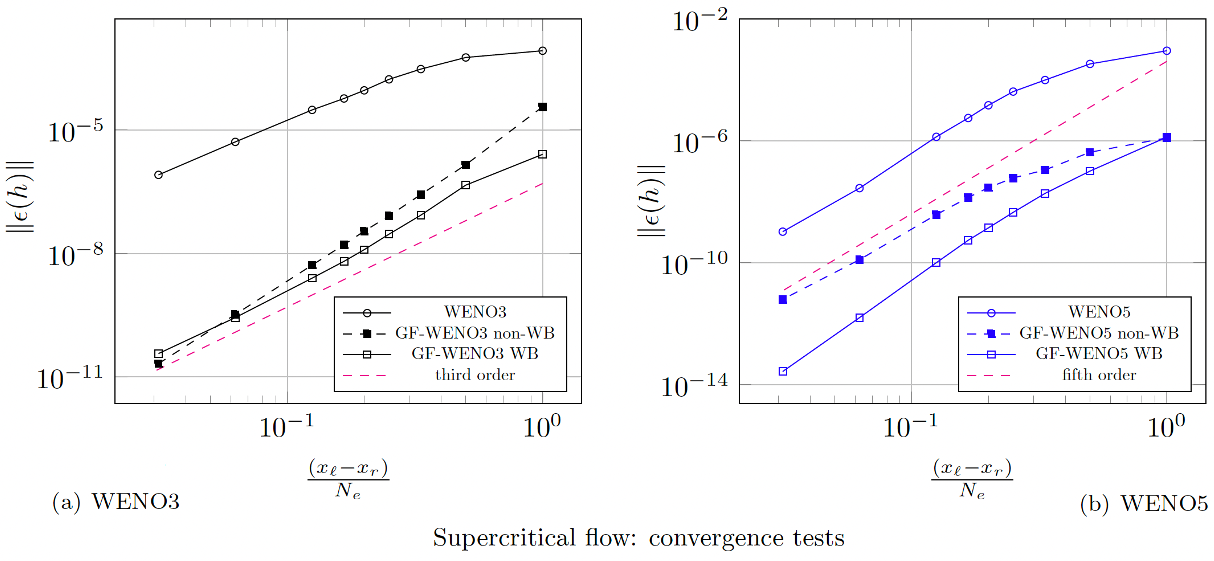
\includegraphics[width=0.6\textwidth]{./GF-FV-WENO-conv}
\end{center}
} 

\only<4>{
{\sf\small Small perturbation of steady state}\\
\begin{center}
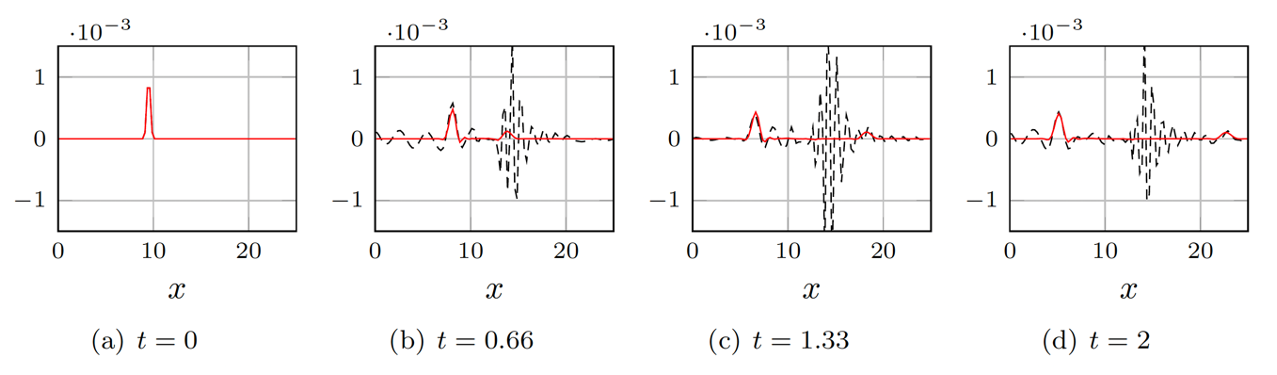
\includegraphics[width=0.9\textwidth]{./GF-WENO-FV-pert} 
\end{center}
} 


\only<5>{
\begin{enumerate}
\item[\textcolor{mblue1}{\Large\checkmark}] \textcolor{black}{No a-priori knowledge of equilibrium, all steady states!}  

\vspace{0.2cm}

\item[\textcolor{mblue1}{\Large\checkmark}] \textcolor{black}{No need of compute the solution of the Cauchy problem .. (maybe for initialization)}  

\vspace{0.2cm}

\item[\textcolor{mblue1}{\Large\checkmark}]  \textcolor{black}{Considerable accuracy enhancements at steady state (3 to 4 orders of magnitude)}

\vspace{0.2cm}

\item[\textcolor{red}{\Large$\times$}]  \textcolor{black}{No super convergence} 

\vspace{0.2cm}

\item[\textcolor{red}{\Large$\times$}]  \textcolor{black}{Very hard to charcterize the steady state and generate one }
\end{enumerate}

\begin{flushright}
$ \overline{R}_i =R_{i-1/2}^+ - \sum_q \omega_q  \int_{x_{i-1/2}}^{x_q} S({\color{red}U_i(x)},\varphi(x)) dx$
\end{flushright}
}




\end{frame}
 
 
 \begin{frame}[t]{
\includegraphics[width=0.3cm]{circle1} Global Flux Quadrature  with WENO approximation} 
\MyLogoa

 We seek solutions of the hyperbolic system of balance laws

\only<1-3>{\begin{equation}
	\partial_tU+\partial_x F(U)=  S(U)\partial_xH   \nonumber
	\vspace{0.25cm}
\end{equation}}

\only<4-6>{\begin{equation}
	\partial_tU+\partial_x \dfrac{U^2}{2}=  S(U) \partial_xH     \nonumber
	\vspace{0.25cm}
\end{equation}}
\only<7->{\begin{equation}
	\partial_t\bigg[\begin{array}{c} h\\hu\end{array}\bigg]+\partial_x\bigg[\begin{array}{c} hu\\hu^2 + gh^2/2\end{array}\bigg]=  - \bigg[\begin{array}{c} 0\\h\end{array}\bigg] b'(x)   \nonumber
%	\vspace{0.25cm}
\end{equation}}

{\bf \textsf{New approach}} 


\only<1-2>{ \begin{equation*} 
 \dfrac{d U_i}{dt} + \dfrac{1}{\Delta x} \left( \widehat{G}_{i+1/2} - \widehat{G}_{i-1/2}   \right)   = 0  \nonumber
 \vspace{0.35cm}
\end{equation*}}
 
 \only<2>{
 
 \begin{enumerate}
 \item  \sout{Reconstruct  WENO polynomials  $U_i(x)$}
 
 \vspace{0.15cm}
 
 \item  Compute  nodal  source primitive $ R_i =R_{i-1} - \Delta x \sum_q \omega_q  S(U_{i-q},\varphi(x_{i-q}))$
 
  \vspace{0.15cm}
  
   \item  \sout{Compute  cell averaged fluxes  $ \overline{F}_i =  \sum_q \omega_q F({\color{red}U_i(x_q)},\varphi(x_q)) dx$}

  \vspace{0.15cm}
    
 \item  Reconstruct  WENO polynomials  $G_{i+1/2}^{\pm}(x)= (F+R)^{\pm}_{i+1/2}(x)$ 
 
  \vspace{0.15cm}
  
 \item  Compute upwind fluxes $\widehat{G}_{i+1/2} = P^+_{i+1/2} G^-_{i+1/2}(x_{i+1/2}) + P^-_{i+1/2} G_{i+1/2}^+(x_{i+1/2})$
 \end{enumerate}
 }

\only<3>{
\begin{block}{Main result}
 {\bf Proposition} (Discrete steady state). {\it     The  WENO-FD scheme with  global flux quadrature 
 preserves exactly \underline{continuous} discrete  steady states $U^*_i =U(F_i)$ with $F$  obtained by integrating the ODE
 $$
 F' = S(U(F)) \partial_x H 
 $$ 
using the  multi-step ODE integrator with weights $\{\omega_q\}_{q\ge 0}$  %\footnote{See e.g.  Theorem 7.10 in Hairer, Wanner and Norset, Solving Ordinary Differential Equations I., Springer 1993}:   
on   spatial slabs of size $\hh$. \\[2.pt]

If $U(F)$ is a one to one mapping,    $U^*(x)$  
 verifies the  consistency estimates of the multi-step scheme.
 }  
 
 \end{block}
 
 \vspace{0.5cm}
 
 \begin{flushright}
{\rm Multi-step schemes so far: Adams methods AB$n$ and AM$n$}
\end{flushright}
} 

 \only<4>{
For $S(U)=U^2$ and $H(x)=x$ exact steady state $u=e^x$ \\[10pt]


\begin{minipage}{0.5\textwidth}
\centering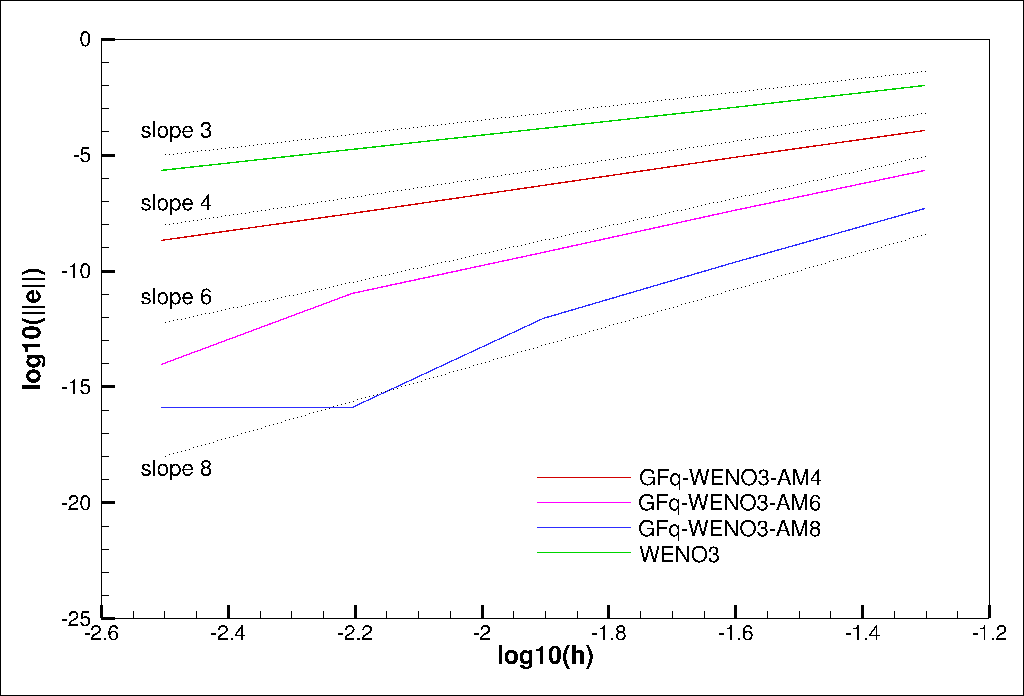
\includegraphics[width=0.8\textwidth]{../figs/WENO-FD/figures/Burgers/convergence_steady/convburg-weno3} 
\end{minipage}\hfill
\begin{minipage}{0.5\textwidth}
\centering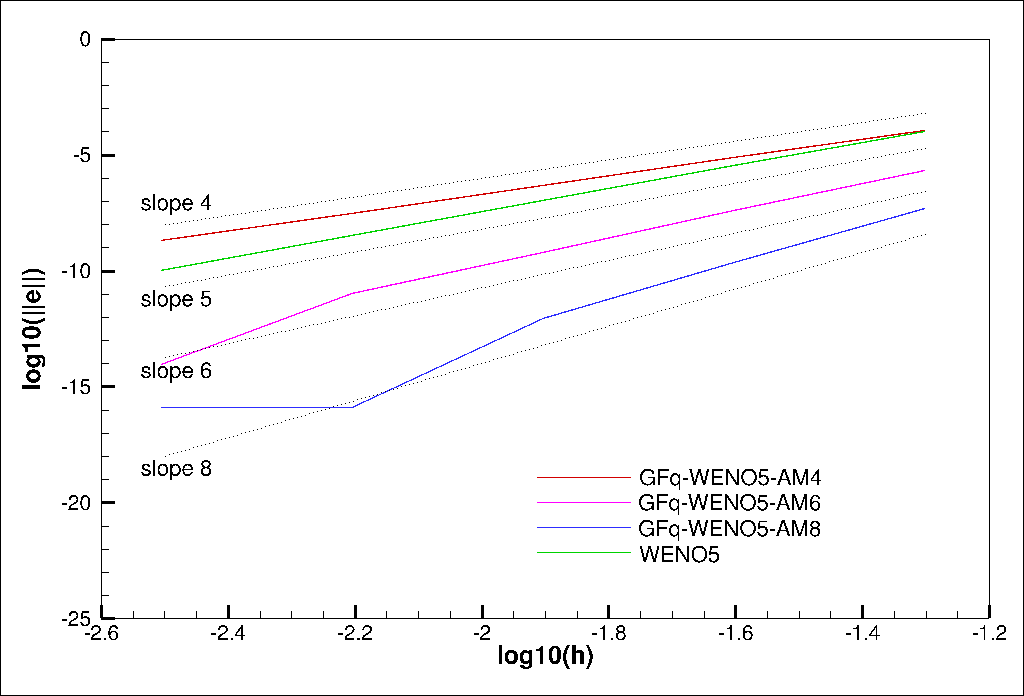
\includegraphics[width=0.8\textwidth]{../figs/WENO-FD/figures/Burgers/convergence_steady/convburg-weno5}
\end{minipage}
} 

\only<5>{
For $s(U)=U^2$ and $\varphi=x+100\sin x$   \\[5pt]


\begin{minipage}{0.5\textwidth}
\centering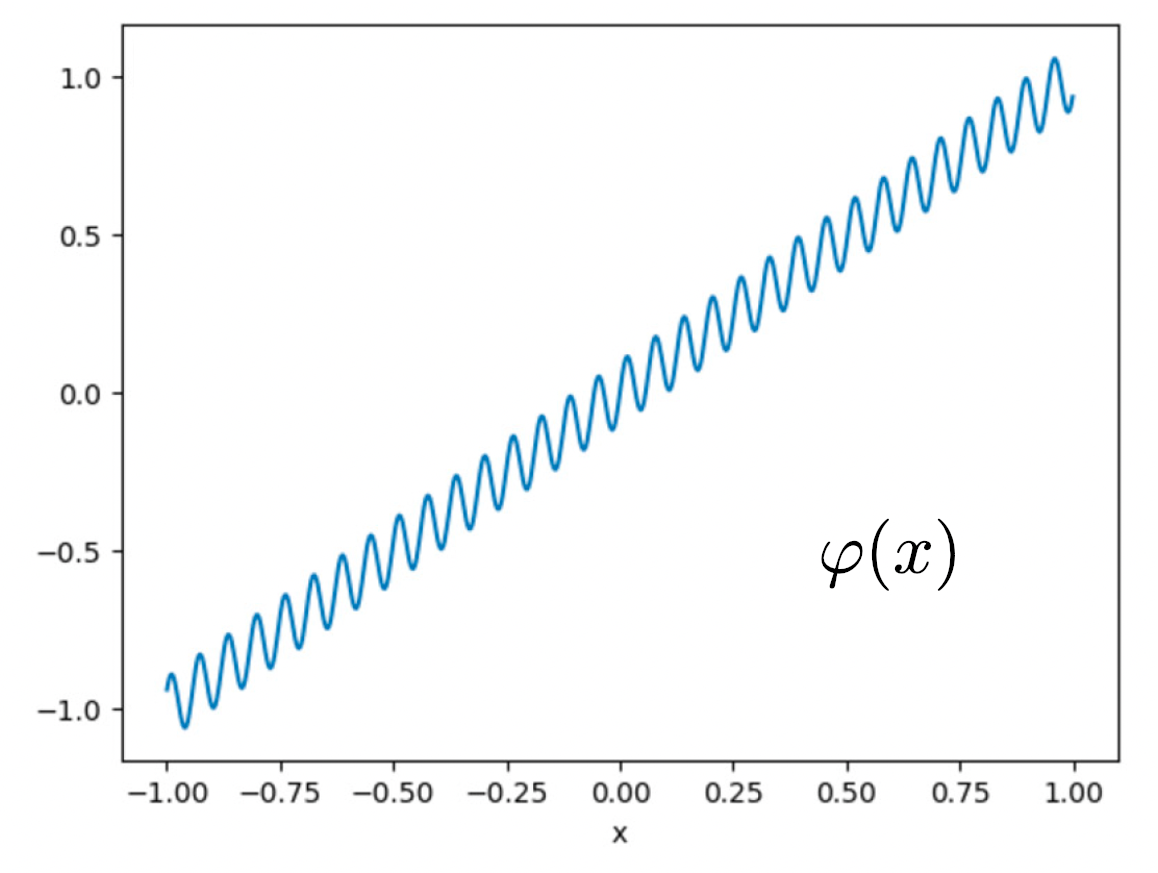
\includegraphics[width=0.8\textwidth]{../figs/WENO-FD/figures/Burgers/perturbations/oscillation} 
\end{minipage}\hfill
\begin{minipage}{0.5\textwidth}
\centering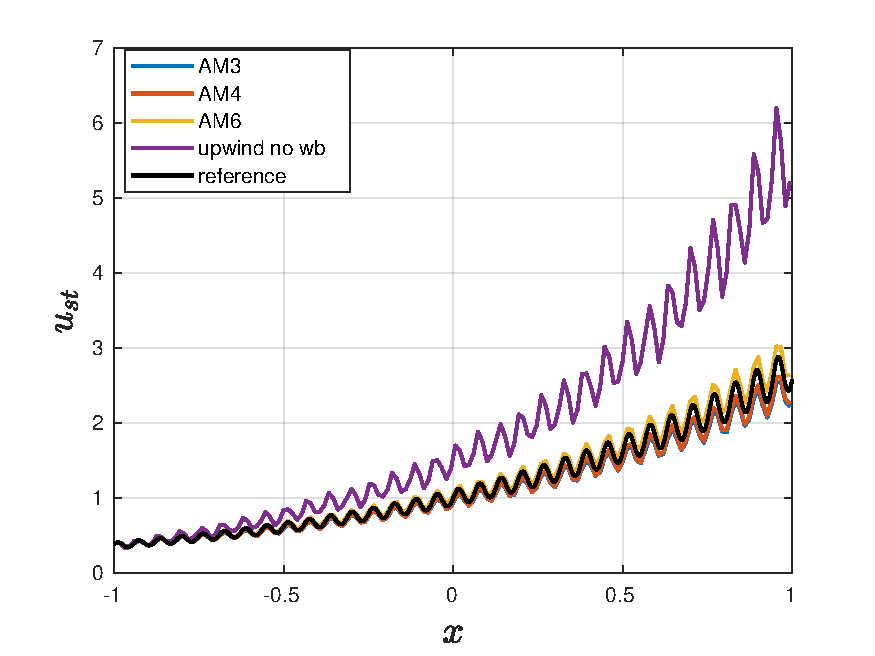
\includegraphics[width=0.85\textwidth]{../figs/WENO-FD/figures/Burgers/perturbations/weno3_AM_stationary_n150} 
\end{minipage}
} 


\only<6>{
For $S(U)=u^2$ and $H=x+100\sin x$ + top hat of perturbation $\delta u=0.2\chi_{[-0.7,-0.5]}$    \\[5pt]


\begin{minipage}{0.5\textwidth}
\centering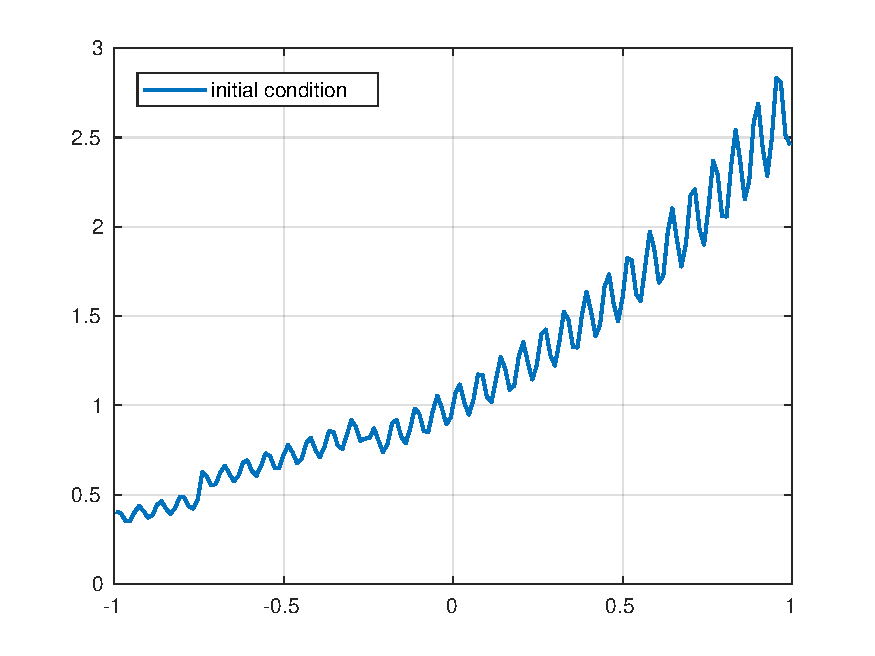
\includegraphics[width=0.8\textwidth]{../figs/WENO-FD/figures/Burgers/perturbations/initial_cond_DISC_n150} 
\end{minipage}\hfill
\begin{minipage}{0.5\textwidth}
\centering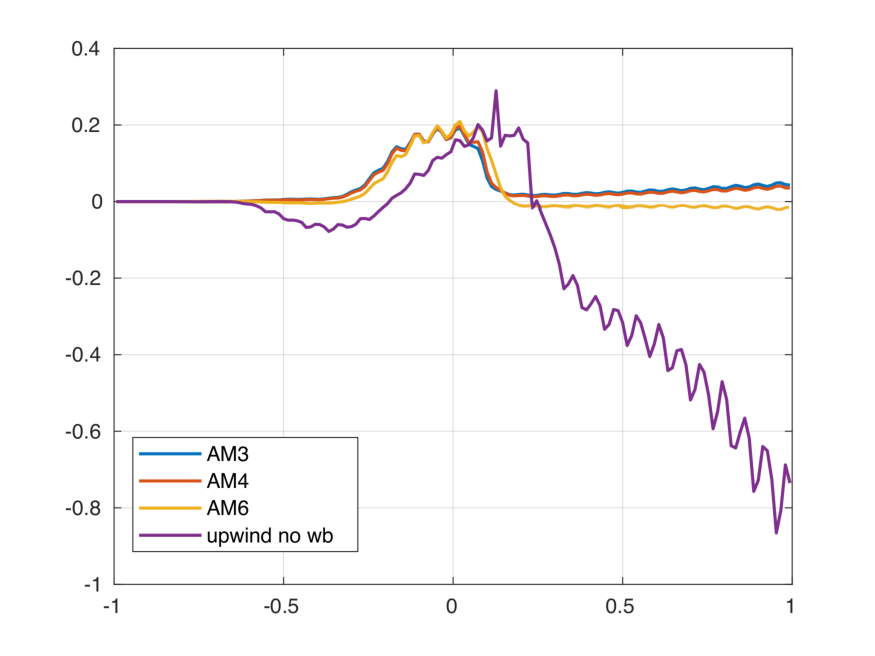
\includegraphics[width=0.85\textwidth]{../figs/WENO-FD/figures/Burgers/perturbations/weno3_AM_DISC_n150} 
\end{minipage}
}

\only<7>{
	For $S(U)=u^2$ and $H=x+100\sin x$ + top hat of perturbation $\delta u=0.2\chi_{[-0.7,-0.5]}$    \\[5pt]
	
	
	\begin{minipage}{0.5\textwidth}
		\centering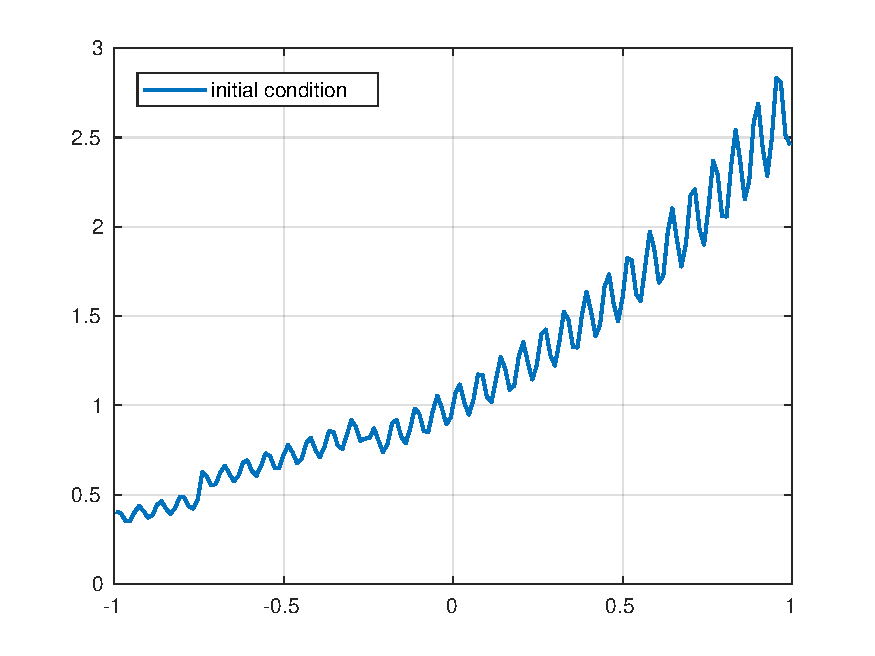
\includegraphics[width=0.8\textwidth]{../figs/WENO-FD/figures/Burgers/perturbations/initial_cond_DISC_n150} 
	\end{minipage}\hfill
	\begin{minipage}{0.5\textwidth}
		\centering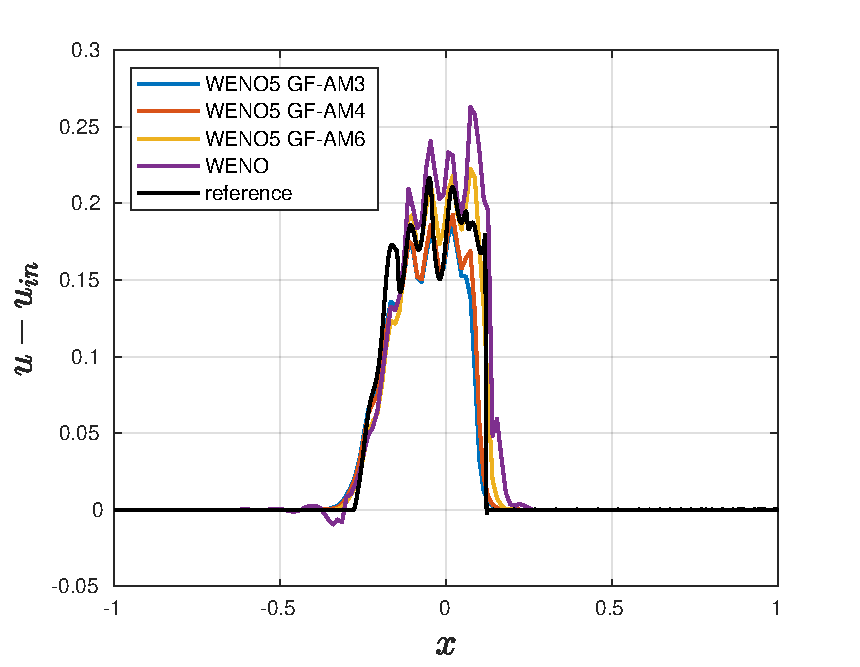
\includegraphics[width=0.85\textwidth]{../figs/WENO-FD/figures/Burgers/perturbations/weno5_AM_DISC_n150} 
	\end{minipage}
}

\only<8>{
	For $S(U)=u^2$ and $H=x+100\sin x$ + top hat of Gaussian perturbation $\alpha=0.005$    \\[5pt]
	
	
	\begin{minipage}{0.5\textwidth}
		\centering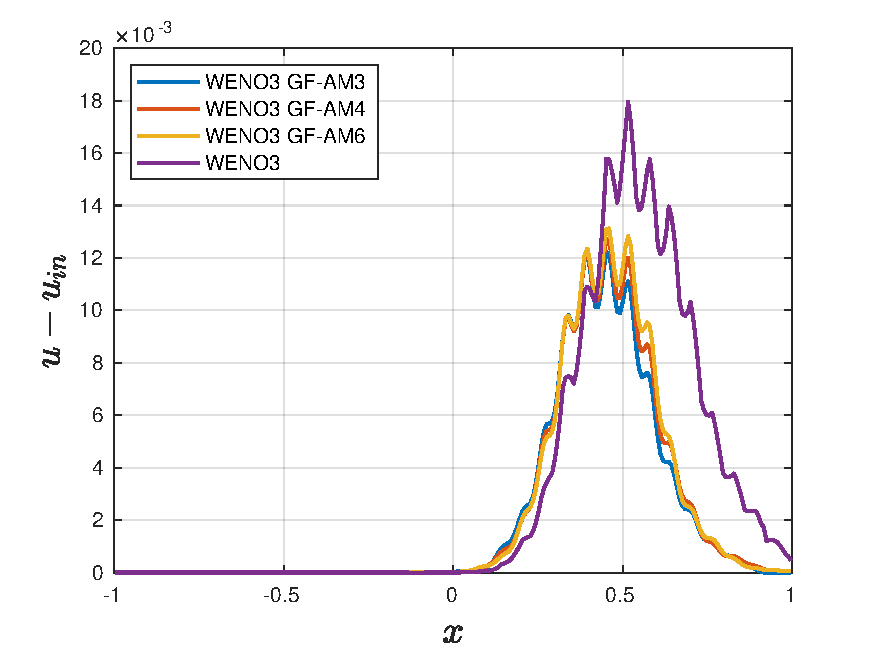
\includegraphics[width=0.85\textwidth]{../figs/WENO-FD/figures/Burgers/perturbations/weno3_AM_error_pert0p005} 
	\end{minipage}\hfill
	\begin{minipage}{0.5\textwidth}
		\centering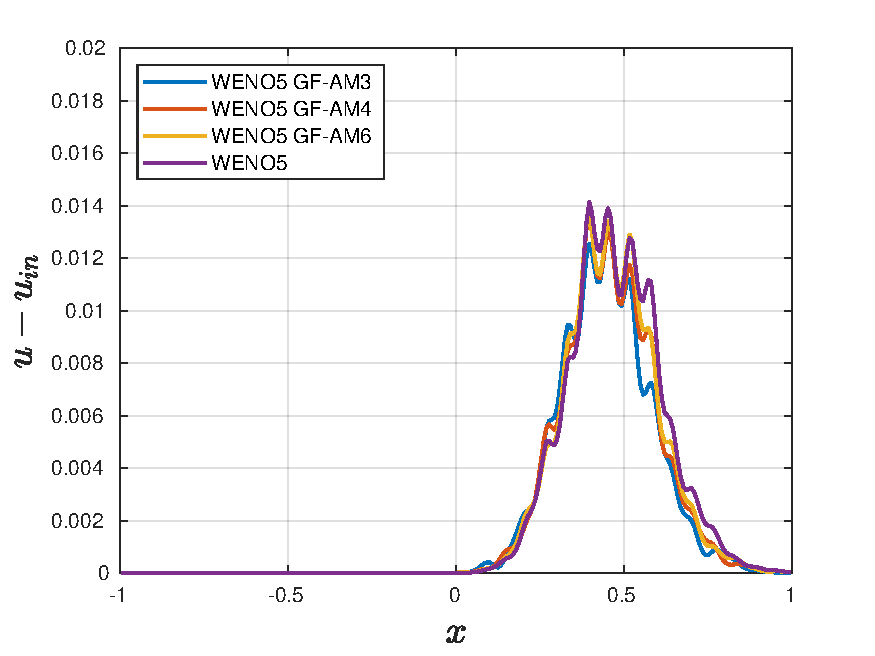
\includegraphics[width=0.85\textwidth]{../figs/WENO-FD/figures/Burgers/perturbations/weno5_AM_error_pert0p005} 
	\end{minipage}
}

\only<9>{
	For $S(U)=u-1$ and $H(x)=e^{-(x-x_0-ct)^2}$, $u(x)=e^{-(x-x_0-ct)^2}.$ The wave is centered at $x_0=0.5$.   \\[5pt]
	
	
	\begin{minipage}{0.5\textwidth}
		\centering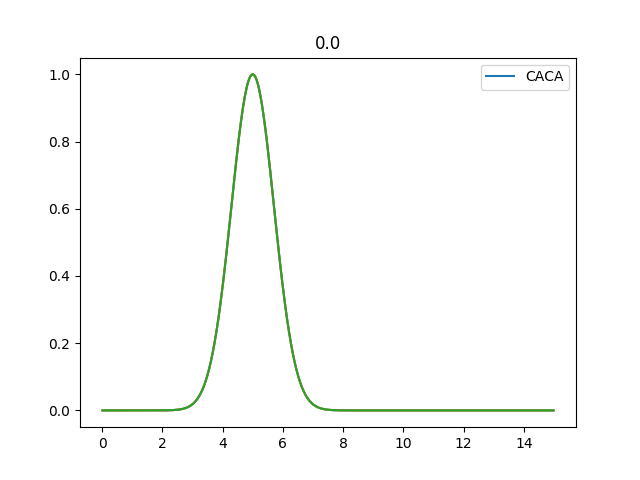
\includegraphics[width=0.8\textwidth]{../figs/WENO-FD/figures/Burgers/MMS/initial} 
	\end{minipage}\hfill
	\begin{minipage}{0.5\textwidth}
		\centering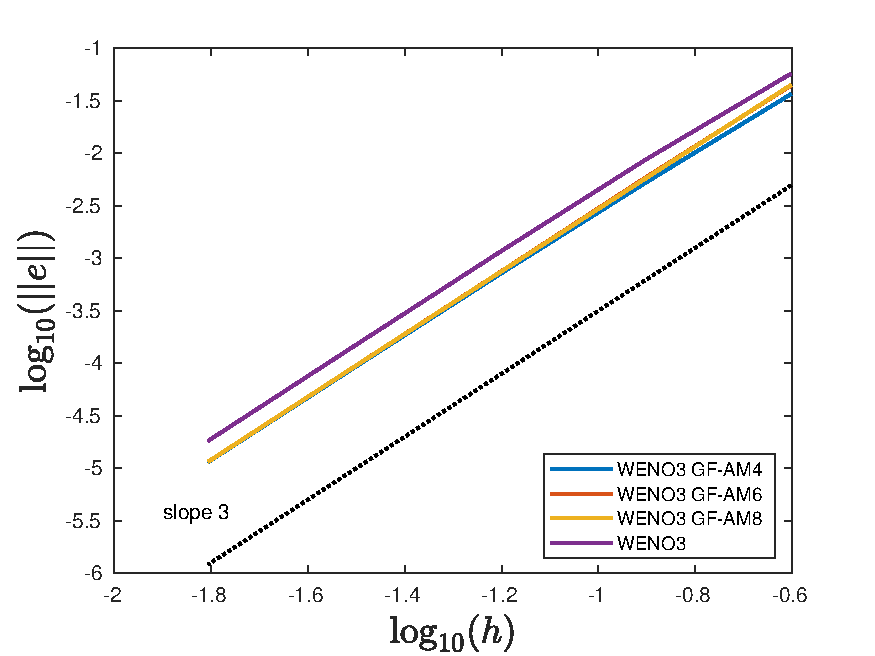
\includegraphics[width=0.85\textwidth]{../figs/WENO-FD/figures/Burgers/MMS/weno3_AM_MMS_conv} 
	\end{minipage}
}

\only<10>{
	For $S(U)=u-1$ and $H(x)=e^{-(x-x_0-ct)^2}$, $u(x)=e^{-(x-x_0-ct)^2}.$ The wave is centered at $x_0=0.5$.   \\[5pt]
	
	
	\begin{minipage}{0.5\textwidth}
		\centering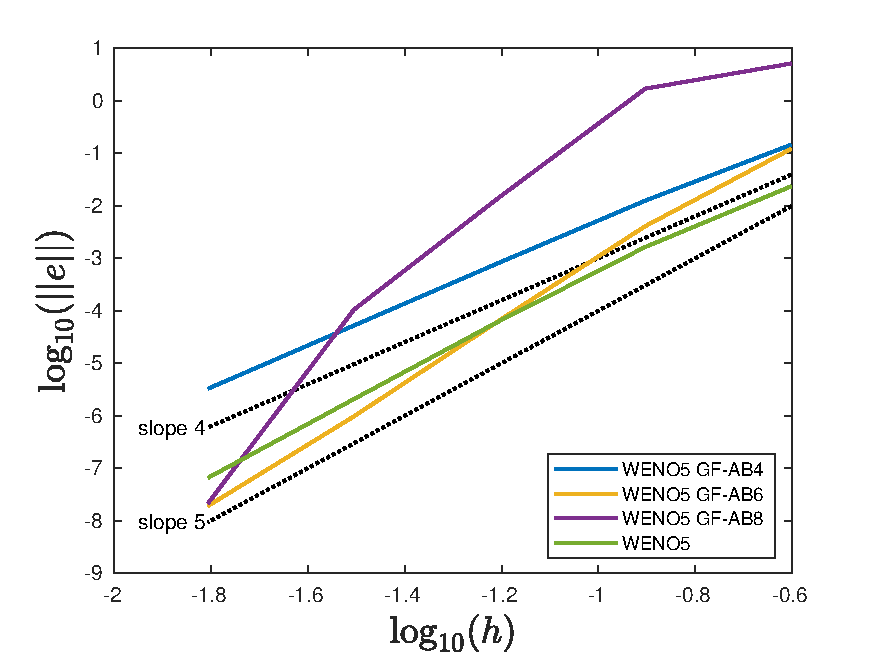
\includegraphics[width=0.8\textwidth]{../figs/WENO-FD/figures/Burgers/MMS/weno5_AB_MMS_conv} 
	\end{minipage}\hfill
	\begin{minipage}{0.5\textwidth}
		\centering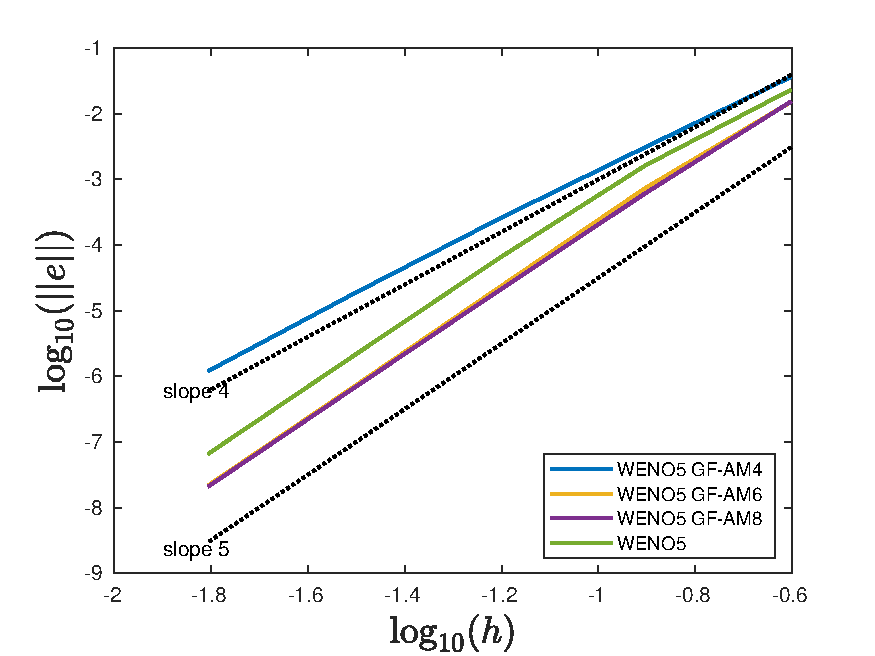
\includegraphics[width=0.85\textwidth]{../figs/WENO-FD/figures/Burgers/MMS/weno5_AM_MMS_conv} 
	\end{minipage}
}


\only<11>{
	For $S(U)=u-1$ and $H(x)=e^{-(x-x_0-ct)^2}$, $u(x)=e^{-(x-x_0-ct)^2}.$ The wave is centered at $x_0=0.5$.   \\[5pt]
	
	
	\begin{minipage}{0.5\textwidth}
		\centering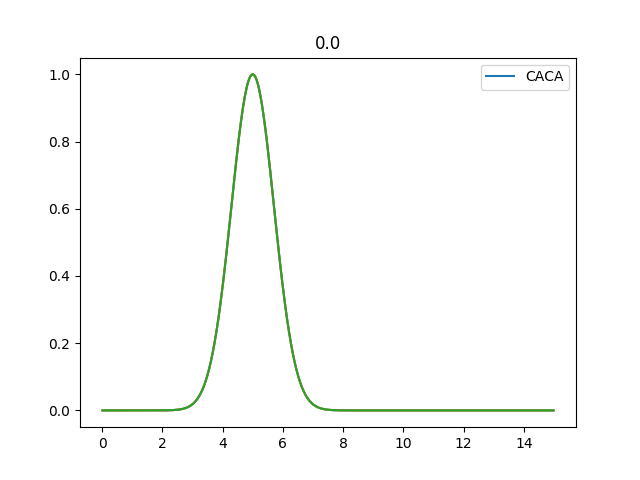
\includegraphics[width=0.8\textwidth]{../figs/WENO-FD/figures/Burgers/MMS/initial} 
	\end{minipage}\hfill
	\begin{minipage}{0.5\textwidth}
		\centering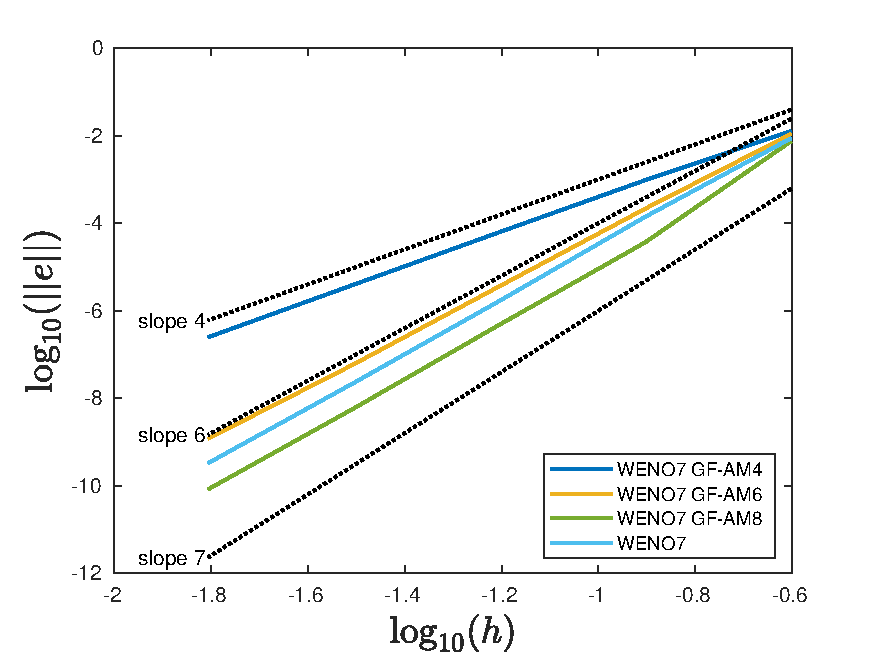
\includegraphics[width=0.85\textwidth]{../figs/WENO-FD/figures/Burgers/MMS/weno7_AM_MMS_conv} 
	\end{minipage}
} 
 
\only<12>{
\begin{minipage}{0.4\textwidth}
Supercritical flow on a smooth hump\\
\centering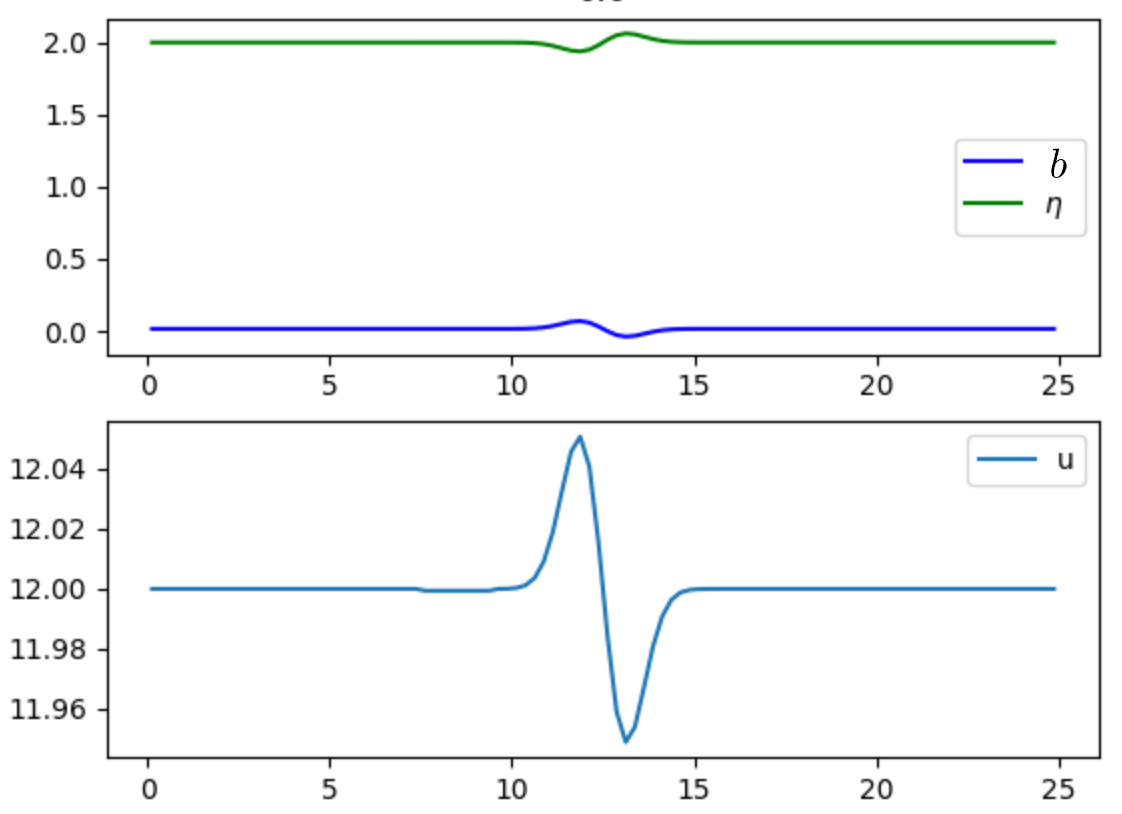
\includegraphics[width=\textwidth]{../figs/WENO-FD/figures/SW/Supercritical/super-ini} 
\end{minipage}\hfill
\begin{minipage}{0.6\textwidth}
\centering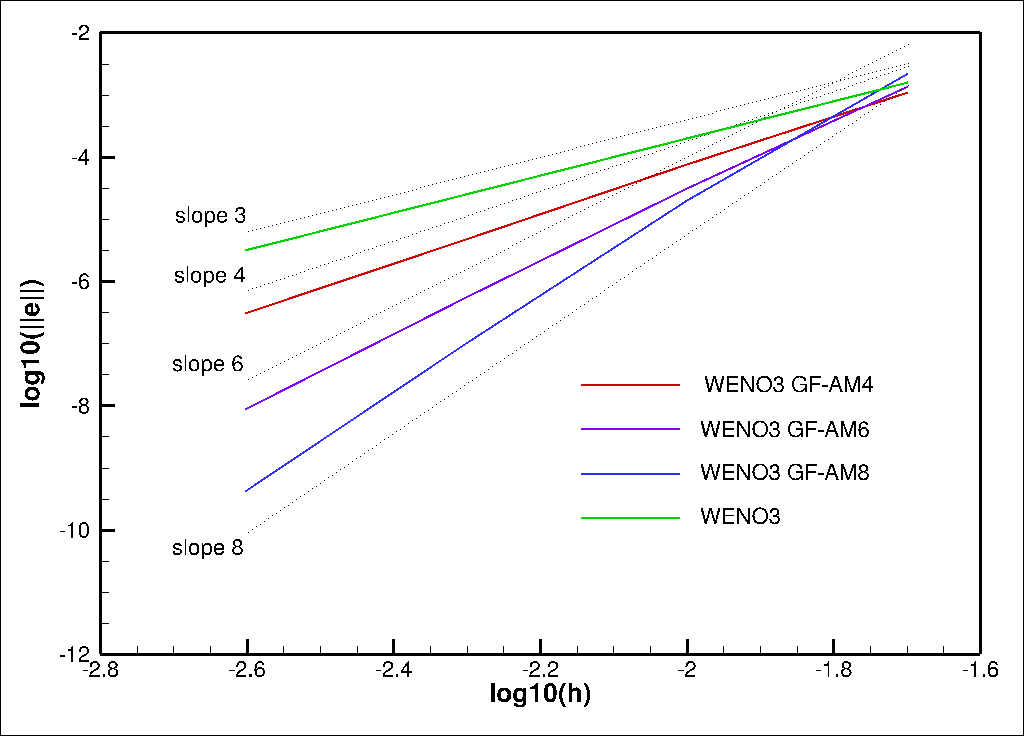
\includegraphics[width=0.8\textwidth]{../figs/WENO-FD/figures/SW/Supercritical/conv} 
\end{minipage}
}

\only<13>{
\begin{minipage}{0.5\textwidth}
\centering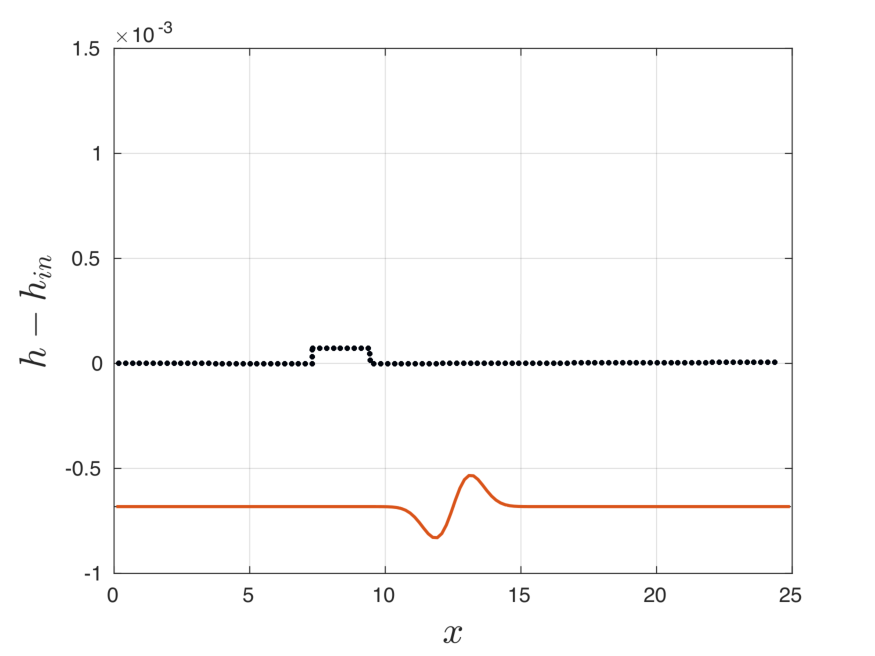
\includegraphics[width=0.9\textwidth]{../figs/WENO-FD/figures/SW/perturbations/weno3_sup_DISCsmall_n100_error_ini}
\end{minipage}\hfill
\begin{minipage}{0.5\textwidth}
\centering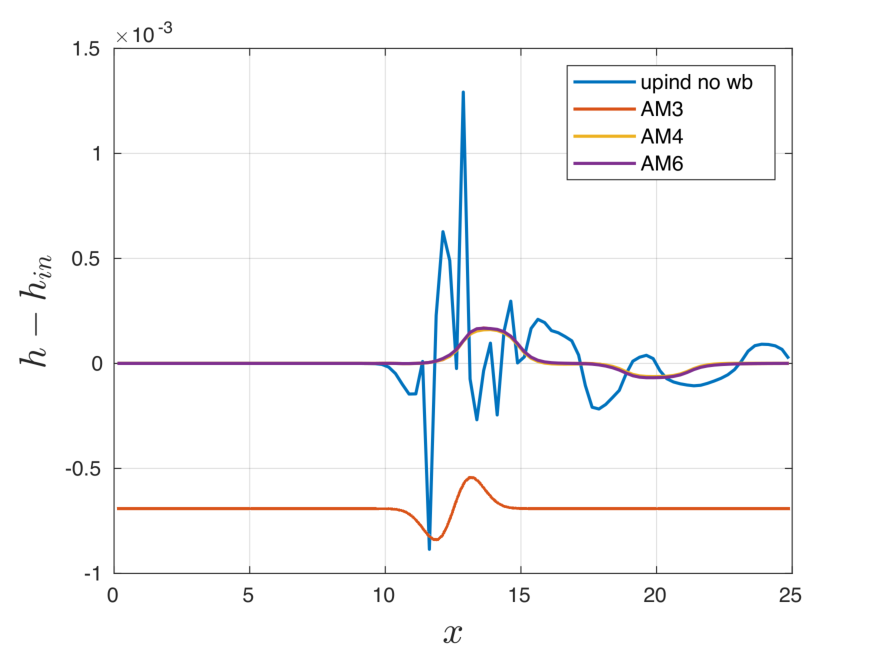
\includegraphics[width=0.9\textwidth]{../figs/WENO-FD/figures/SW/perturbations/weno3_sup_DISCsmall_n100_error_h} 
\end{minipage}
}


\only<14>{
\begin{minipage}{0.5\textwidth}
\centering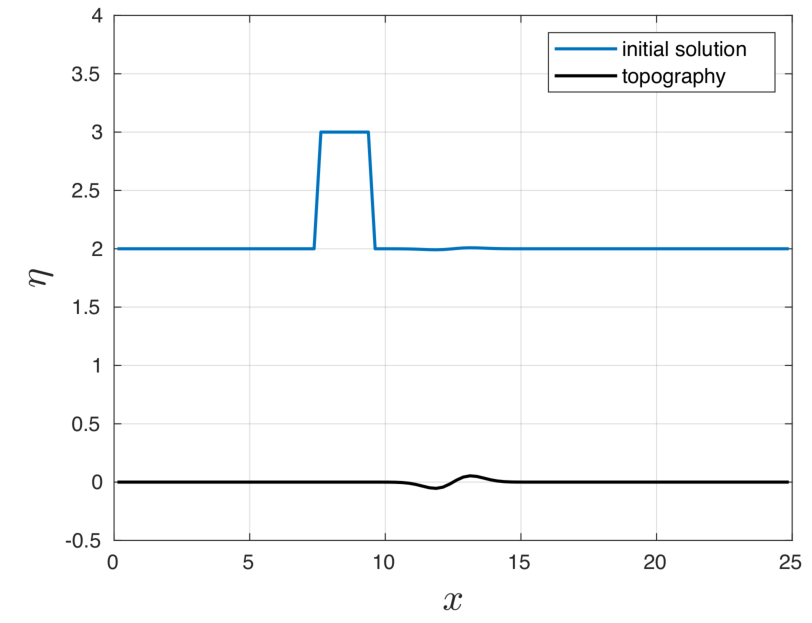
\includegraphics[width=0.9\textwidth]{../figs/WENO-FD/figures/SW/perturbations/initial_discbig}
\end{minipage}\hfill
\begin{minipage}{0.5\textwidth}
\centering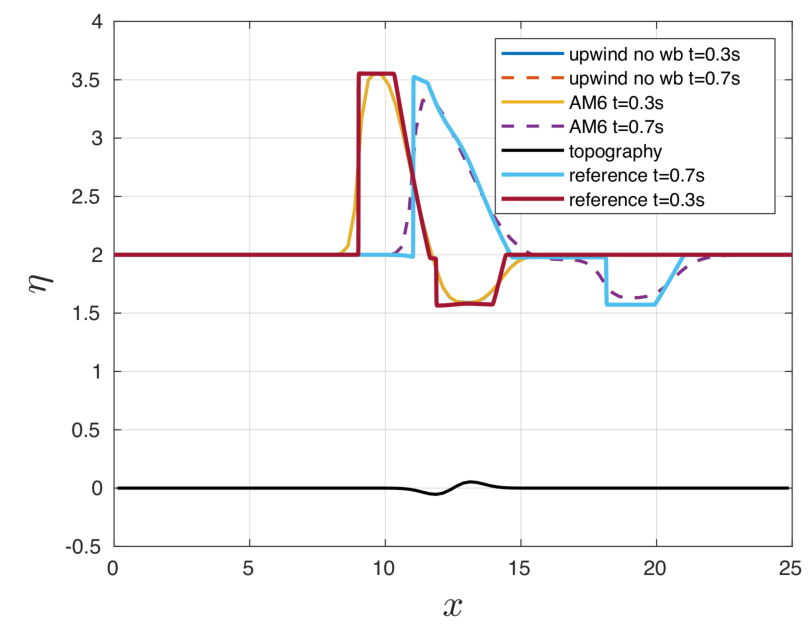
\includegraphics[width=0.9\textwidth]{../figs/WENO-FD/figures/SW/perturbations/weno3_evolution_upAM61} 
\end{minipage}
}


\only<15>{
	\begin{minipage}{0.4\textwidth}
		Subcritical flow on a smooth hump\\
		\centering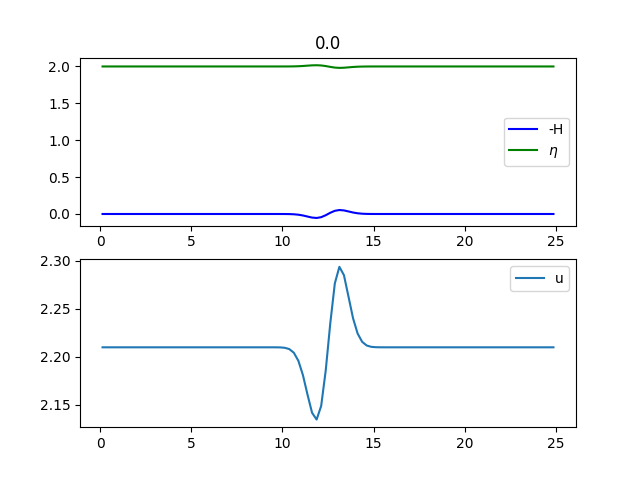
\includegraphics[width=\textwidth]{../figs/WENO-FD/figures/SW/Subcritical/initial_con} 
	\end{minipage}\hfill
	\begin{minipage}{0.6\textwidth}
		\centering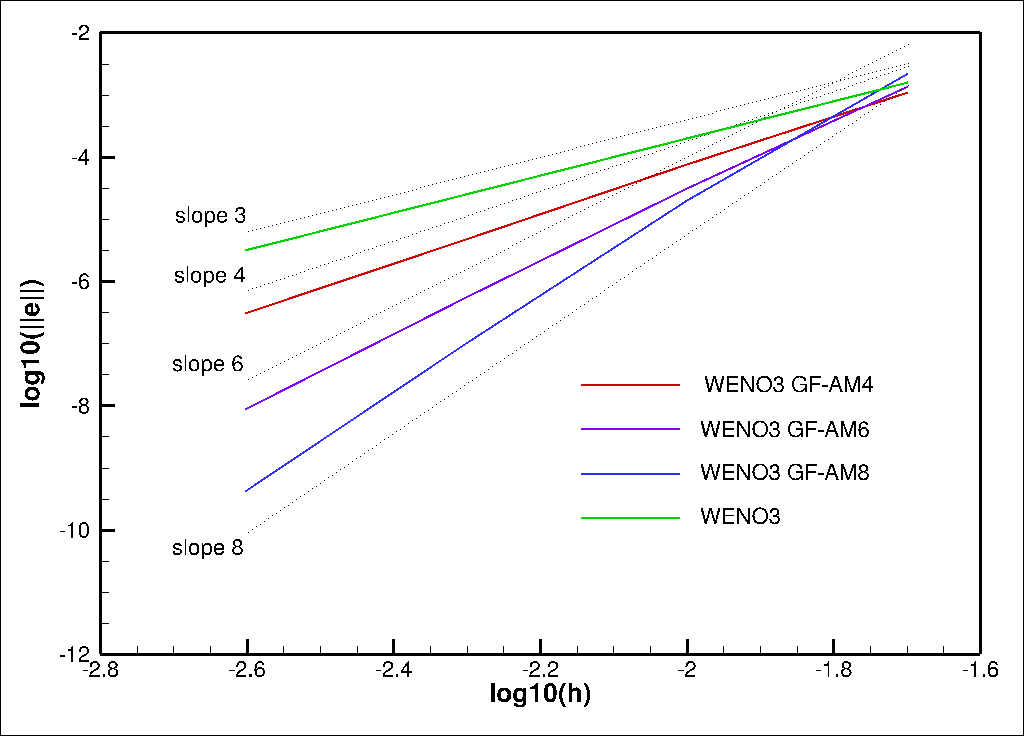
\includegraphics[width=0.8\textwidth]{../figs/WENO-FD/figures/SW/Supercritical/conv} 
	\end{minipage}
}


\only<16>{

\vspace{0.5cm}

\begin{enumerate}
\item[\textcolor{mblue1}{\Large\checkmark}] \textcolor{black}{No a-priori knowledge of equilibrium, all steady states!}    

\vspace{0.2cm}

\item[\textcolor{mblue1}{\Large\checkmark}] \textcolor{black}{No need of compute the solution of the Cauchy problem .. (maybe for initialization)}  

\vspace{0.2cm}

\item[\textcolor{mblue1}{\Large\checkmark}]  \textcolor{black}{Convergence at steady state arbitrarily accurate by changing ODE weights} 

\vspace{0.2cm}

\item[\textcolor{mblue1}{\Large\checkmark}]   \textcolor{black}{Discrete initial state can be generated}

\vspace{0.2cm}

\item[\textcolor{red}{\Large$\times$}]   \textcolor{black}{Non-compact quadrature }
\end{enumerate}

}

\end{frame}
% 
 
      


\section[End]{Conclusion and perspectives}

  

 \begin{frame}{This is the last slide} 
\MyLogoa


\begin{block}{Take home message}
\begin{itemize}
\item GFq in 1D:  clever   quadrature of
the source based on high order ODE integrators

\vspace{0.1cm}

\item Tremendous error reduction  at stady-state (super-covergence)

\vspace{0.1cm}


\item  In one dimension  discrete equilibria can be generated a-priori if necessary   with the ODE solver

 
 \end{itemize}
 \end{block} 

\begin{alertblock}{Future}
\begin{itemize}
\item   Sonic points ? 

\vspace{0.1cm}

\item discontinuous  data ?

\vspace{0.1cm}

\item adaptive ODE weights

\vspace{0.1cm}

\item multiD 
 \end{itemize}
 \end{alertblock} 
 \end{frame}



 

%
% \begin{frame} 
%\MyLogoa
%
% 
%\begin{flushright}
%\testsf{\HUGE THX !}
%%\includegraphics[width=0.3\textwidth]{spasibo}
%\end{flushright}
% 
  
%  \end{frame}

  
 
\end{document}


